\documentclass{beamer}

\usepackage[T1]{fontenc}
\usepackage[latin1]{inputenc}
\usepackage{ngerman}
\usepackage{graphics}
\usepackage{pgf}
\usepackage{multimedia}
\usepackage{color}

%\definecolor{darkyellow}{rgb}{50,30,0}

\title{Yeminy Chat System}
\author{Ulf Gebhardt, Konstantin Rupp, Kai Hofmann, Oliver Kaleja}
\date{17 Jannuar 2007}

\usetheme{Frankfurt}

\begin{document}

  \frame{\titlepage}

\section{Inhalt}

  \frame{\frametitle{Inhalt}
  			 \tableofcontents} 

\section{Das Funktionsprinzip}

  \frame{\begin{center}
  			 \huge{Das Funktionsprinzip}
  			 \end{center}}
  			 
  \frame{\frametitle{�bersicht}
         \begin{center}         
  			   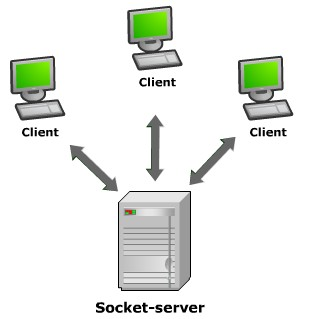
\includegraphics[height=7cm]{img/client_server.jpg}
  			 \end{center}}

  \frame{\frametitle{Das Protokoll}
  			 Vorteile:\\
  			 \begin{itemize}
  			   \item{Standardisierung}
  			   \item{Unabh�ngige Entwicklungsteams}
  			   \item{Verschiedene Entwicklungsteams}
  			 \end{itemize}
  			 Anforderungen:\\
  			 \begin{itemize}
  			   \item{Aktuell}
  			   \item{Erweiterbar}
  			   \item{�bersichtlich}
  			   \item{Gute Dokumentation}
  			 \end{itemize}}
  			 
  \frame{\frametitle{Der Server}
  			 Anforderungen:\\
  			 \begin{itemize}  			
  			   \item{Stabil}
  			   \item{Schnell}
  			   \item{Ressourcen schonend}
  			   \item{Aktuellstes Protokoll}
  			   \item{Systemunabh�ngig}  			  
  			 \end{itemize}}  
  			 
  \frame{\frametitle{Die Clients}
  			 Anforderungen:\\
  			 \begin{itemize}  			
  			   \item{Benutzerfreundlich}
  			   \item{Aktuell(Aktuellstes Protokoll)}
  			   \item{Ansprechendes Layout}
  			 \end{itemize}}

\section{YChat-Protokoll}

  \frame{\begin{center}
  			 \huge{YChat-Protokoll}
  			 \end{center}}

  \frame{\frametitle{Befehlsaufbau}
         \begin{center}
           \itshape{\footnotesize{Befehlname Operator Befehlsvariable1 Operator Befehlsvariable2 Operator...}}\\
         \end{center}
         \begin{itemize}
         \item{Operator im YChat-Protokoll ist ;}
         \item{Keine definierte L�nge der Befehle -> Flexibilit�t}
         \item{Nach jedem Befehl ein Return zur Trennung}
         \end{itemize}
         }
         
  \frame{\frametitle{Befehlsliste}  		
         \large{Einige Befehle:}
         \begin{itemize}
  			   \item{login;UserID;PW;}
  			   \item{setallowadd;1/0;}
  			   \item{getallowadd;UserID;}
  			   \item{setstatus;StatusNumber;(status-text)}
  			   \item{getstatus;UserID;}
  			   \item{setstatustext;statustext{text}}
  			   \item{getstatustext;UserID;}
  			   \item{setpw;OldPW;NewPW;}
  			   \item{setnick;NewNick}
  			 \end{itemize}}
  			 
  \frame{\frametitle{Einschr�nkungen}
         \begin{center}
  			 \large{Reservierte Zeichen:\\}
  			 \begin{itemize}
  			   \item{Return}
  			   \item{;}
  			   \item{| (Nur teilweise)}
  			 \end{itemize} 
  			 \end{center}}
  			 
  \frame{\frametitle{Aktuelles}
         \begin{center}
         Ver�ffentlicht: Protokollversionen 0.35 und 0.36\\
         In Arbeit: Protokollversion 0.37\\
  			 \end{center}}

\section{YChat-Server}

  \frame{\begin{center}
  			   \huge{YChat-Server}
  			 \end{center}  
  			 \begin{center}
    			 \tiny{Im Moment 3423 Code-Zeilen}
  			 \end{center}}
  			 
  \frame{\frametitle{Struktur}
         %\begin{center}
           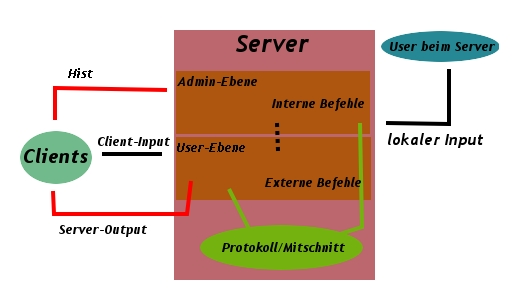
\includegraphics[width=11cm]{img/server-strucktur.jpg}}
         %\end{center}}
         
  \frame{\frametitle{Interne Befehle}
  			 \large{Einige Befehle:}
         \begin{itemize}
  			   \item{listallusers}
  			   \item{showuserinfo;UserID;}
  			   \item{kickuser;UserID;}
  			   \item{banuser;UserID;}
  			   \item{restartserver}
  			   \item{shutdownserver}
  			   \item{allowinet}
  			   \item{denylan}
  			   \item{loaduserdb}
  			 \end{itemize}}
  
  \frame{\frametitle{Fehler/Probleme}
         \large{Aktuell:}
         \begin{itemize}        
           \item{Nicht alle Ereignisse werden geloggt}
           \item{Zeichenersetzung}
           \item{Nicht flexibel genug}
           \item{Abstimmung auf einen Client}
           \item{schlechtes Englisch}
         \end{itemize}}
         
  \frame{\frametitle{Planung/M�glichkeiten}
         \begin{itemize}
  			   \item{Portierung nach Delphi-Konsole}
  			   \item{Portierung nach C++/FreePascal}  			   
  			   \item{DelphiScript implementieren}
  			 \end{itemize}}

\section{YChat-Client}

  \frame{\begin{center}
  			   \huge{YChat-Client}
  			 \end{center}
  			 \begin{center}  
  	  		 \tiny{Im Moment 1820 Code-Zeilen}
  	 		 \end{center}}
  	 		 
 \frame{\frametitle{Struktur}
         %\begin{center}
           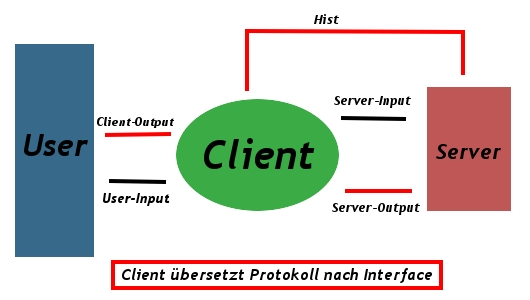
\includegraphics[width=11cm]{img/client-strucktur.jpg}}
         %\end{center}} 		 
         
  \frame{\frametitle{Layout}
         \begin{center}
           Ein ansprechendes Layout soll �ber TBX realisiert werden.\\
           \begin{center}
           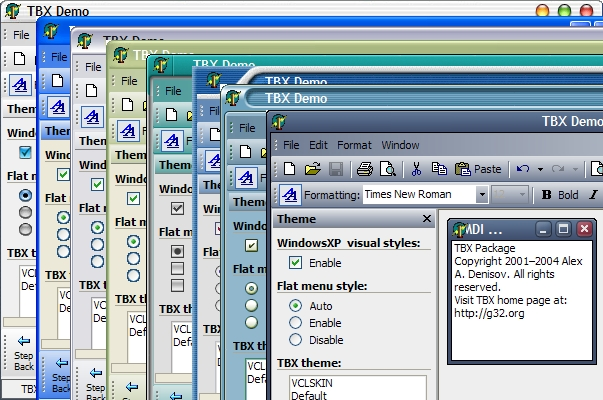
\includegraphics[height=4cm]{img/tbx.jpg}
           \end{center}
         \end{center}}
         
  \frame{\frametitle{Fehler/Probleme}
         \large{Aktuell:}
         \begin{itemize}
           \item{GIFs werden nicht immer geladen}
           \item{Ungetestet}
           \item{Protokoll nicht vollst�ndig umgesetzt}
           \item{Konfiguration}
         \end{itemize}}

  \frame{\frametitle{Planung/M�glichkeiten}
         \begin{itemize}
           \item{Portierung nach Miranda-Plugin}
           \item{TBX implementieren}
         \end{itemize}}  			
  			
\section{Live-Demonstration}

   \frame{\begin{center}
            \huge{Es folgt nun eine kurze Demonstration des YChat-Systems.}
          \end{center}}
  			
\section{Danksagung}

  \frame{
  			 \begin{center}
         Dank gilt dem Yeminy-Team. Von allen ist aber Ole Hoppe hervorzuheben, der uns
         tatkr�ftig beim Schreiben des Clients unterst�tzt hat.
         \end{center}
                 
         \begin{center}
           \Large{Danke f�r Ihre Aufmerksamkeit.}
         \end{center}          
         
         \begin{center}
         Besuchen Sie bei weiterem Interesse an dem Thema
         \textit{http://www.yeminy.redpro.de} .
         \end{center}
         \pgfputat{\pgfxy(10,-1.5)}{\pgfbox[right,base]{
\includegraphics[height=1.5cm]{img/linux.jpg}}}
\pgfputat{\pgfxy(0,-1.5)}{\pgfbox[left,base]{
\includegraphics[height=1cm]{img/latex.jpg}}}}

\end{document}
